\documentclass[12pt]{report}
\usepackage[margin=1in,footskip=0.25in]{geometry}
\setlength{\parskip}{\baselineskip}
\setlength{\parindent}{0pt}

\usepackage[ruled,vlined]{algorithm2e} %Uses version 3.9
\usepackage{url}
\usepackage{graphicx}
\usepackage{caption}
\usepackage{subcaption}
\usepackage{float}

\newcommand{\TODO}[1]{}
% \renewcommand{\familydefault}{\sfdefault} % use sans-serif font
\usepackage{times}

\begin{document}
\title{Reducing Contention in Concurrent Queues}
\author{Carlos Valera \\
    University of Central Florida \\
    \texttt{cvaleraleon@knights.ucf.edu}}
\date{April 15, 2013}
\maketitle
\begin{abstract}
I introduce the concepts of operation for a new contention management system
for concurrent queues called a MultiQueue. The MultiQueue wraps concurrent
queue algorithms from previous authors, and reduces contention on accesses to
these queues from multiple threads by distributing data across multiple
structure instances. I tested the throughput MultiQueue under various
load conditions and compared the results against previous implementations of
queues without the MultiQueue.
\end{abstract}
\section{Introduction}
%Problem Description
The concurrent queue is a well-studied and practical structure in concurrent
programming. One issue with the concurrent queue is that because queues are an
inherently sequential data-structure, many implementations of concurrent queues
suffer from high contention when under load. I will describe a method for
managing contention between queues to gain performance. I call the structure
which does this a MultiQueue. The method primarily builds on the two lock queue
introduced by Micheal and Scott\cite{michael1996}and tries to improve
concurrency by distributing the work presented to the queue amongst multiple
instances of a two-lock queue structure. 

%History
\section{Algorithms}
%Concepts
The concepts surrounding the MultiQueue are simple enough. The structure keeps
an internal list of concurrent queues and two counters that keep track how many
enqueue and dequeue operations have been made on the MultiQueue. In essence,
the internal list is treated like a circular array based queue of queues, and
the two counters essentially point to the head and tail of this queue. The
intent is to isolate the enqueue and dequeue operations of more complex queue
algorithms so that, on average, each queue has only one producer and one
consumer operating on it. Because of the ordering enforced by the MultiQueue,
all the queues in the circular array constitute a single large queue.

%Pseudocode
\begin{small}
\begin{algorithm}[H]
\SetKwIF{blk}{}{}{}{}{}{}{} % Hacky way to get vline to work properly with blocks
\SetKwFunction{Init}{void initialize}
\SetKwFunction{Enq}{void enqueue}
\SetKwFunction{Deq}{bool dequeue}
\SetKwFunction{ienq}{internalEnqueue}
\SetKwFunction{ideq}{internalDequeue}
\SetKwFunction{iinit}{internalInitialize}
\SetKwFunction{FAA}{fetchAndAdd}
\SetKwFunction{nexttwo}{nextPowerOf2}
\SetKwFunction{ladd}{listAdd}
\SetKw{Continue}{continue}
\SetKw{Struct}{structure}
\SetKwFor{For}{for}{}{}
\SetKwIF{If}{ElseIf}{Else}{if}{}{elif}{else}{}
\SetKwFor{While}{while}{}{}
\SetKwInOut{Input}{input}
\SetKwInOut{Output}{output}
\SetNoFillComment

\caption{Pseudocode defining the operations which can be done on a MultiQueue
         as well as the structure of a MultiQueue.}

\Struct InternalQueue
\blk{}{
    \tcp{The internal structure of this is not important as long as supports
    the concurrent enqueue and dequeue operations}
}

\Struct MultiQueue
\blk{}{
    int num\_queues\;
    int mask \tcp*[r]{Bitmask used to wrap counters}
    uint producer\_counter \tcp*[r]{Tracks the next "empty" spot for a producer}
    uint consumer\_counter \tcp*[r]{Tracks the next "empty" spot for a consumer}
    list queues \tcp*[r]{A list of internal concurrent queues}
}
\BlankLine
\BlankLine
\BlankLine
\BlankLine
\BlankLine

\Input{The multi queue to initialize and the number of queues to initialize it
       for}
\Init{MultiQueue Q, int num\_queues}
\blk{}{
    Q.producer\_counter = Q.consumer\_counter = 0\;
    Q.num\_queues = \nexttwo{num\_queues}\;
    Q.mask = Q.num\_queues$-$1\;
    Q.queues = list()\;
    \For{i=0 \KwTo Q.num\_queues}{
        IQ = InternalQueue\;
        \iinit{IQ}\;
        \ladd{Q.queues, IQ}
    }
}
\BlankLine
\BlankLine
\BlankLine
\BlankLine
\BlankLine

\Input{The multi queue to enqueue into and the item to enqueue}
\Enq{MultiQueue  Q, data\_t\_ptr item}
\blk{}{
    next\_empty = \FAA{Q.producer\_counter, 1}\;
    next\_queue = Q.queues[next\_empty]\;
    \ienq{next\_queue, item}\;
}
\BlankLine
\BlankLine
\BlankLine
\BlankLine
\BlankLine

\Input{The multi queue to attempt to dequeue from and an address to a location
       to store the dequeued item}
\Output{If the queue is empty, false is returned, otherwise true is returned
        and the value of the dequeued item is copied into the address pointed to by
        \it{result}}
\Deq{MultiQueue Q, data\_t\_ptr result}
\blk{}{
    \If(\tcp*[f]{quit if queue is empty}){Q.consumer\_ptr $\ge$ Q.producer\_counter}{
        \Return{false}\;
    }
    next\_empty = \FAA{Q.consumer\_counter, 1}\;
    next\_queue = Q.queues[next\_empty $\&$ Q.mask]\;
    \BlankLine
    \tcp{Keep trying to dequeue an item until one is found. This loop is needed
         to prevent race conditions between a consumer dequeueing and a producer
         enqueueing at the same time}
    \While{$\neg$\ideq{next\_queue, result}}{
        \Continue
    }
    \Return{true}\;
    
}
\end{algorithm}
\end{small}

\section{Correctness}
Typically, each operation of a MultiQueue works in isolation of others. That
is, each thread will acquire one queue to work on, and can generally assume
that it is the only thread working on it. However, there are situations where a
faster thread may wrap around the queue, colliding with a slower thread. In
this circumstance, the correctness of the following sequence of events is
solely dependant on the correctness guarantees of the datastructure that the
MultiQueue is wrapping access to. Because of this, the correctness of the
MultiQueue is fundementally tied to the queue it uses as a base. Nonetheless,
there are still a few guarantees we can make about the MultiQueue.

\begin{enumerate}
\item For every position in the queue list which is greater than the consumer
counter and less than the producer counter, either there is at least one item
in the corresponding queue, or there is a producer performing an enqueue
operation in that slot. 

\item The consumer counter never exceedes the producer counter. This is
prevented by first conditional statement in the dequeue operation. Both
counters are only ever incremented by one, so 
\end{enumerate}

\section{Performance}
\subsection{Setup}
The tests were designed to compare throughput of items through a queue. Each
thread was designated as either a consumer or a producer, and would
continuously cycle through performing its operation on a queue (dequeueing and
enqueueing, respectively), and doing a small amount of work. This cycle was
continued for some amount of time, and the number of items which made it
through the queue were tallied at the end. The number of internal queues used
by the MultiQueue in these tests was set to the maximum of the producer and
consumer threads that would be working on it.

Due to time constraints, I was only able to test two cases: a two-lock queue
adapted from Micheal and Scott's algorithms\cite{michael1996}, and a MultiQueue
with a two-lock queue as the base. All tests were conducted on an Intel Core
i5-2500K CPU, which has four cores. The source code for the implementation of
the algorithms and the tests can be found online at:
\url{https://github.com/cookyt/parallel-multi-queue}

\subsection{Results}
\begin{figure}[H]
    \centering
    \begin{subfigure}[b]{0.45\textwidth}
        \centering
        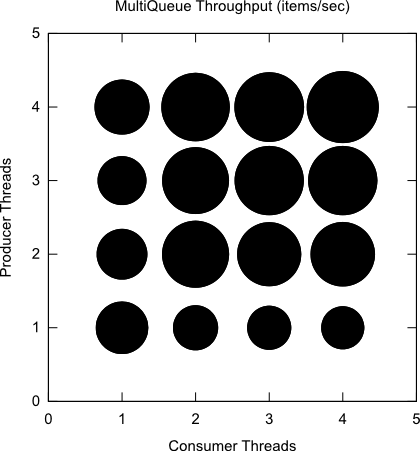
\includegraphics[width=\textwidth]{multiqueue.png}
        \caption{min=1856809, max=5150969}
    \end{subfigure}
    \hfill
    \begin{subfigure}[b]{0.45\textwidth}
        \centering
        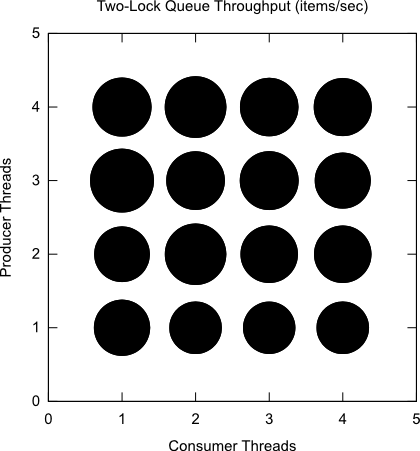
\includegraphics[width=\textwidth]{two-lock.png}
        \caption{min=2707499, max=4027409}
    \end{subfigure}
    \caption{Throughput of the queues when subjected to continuous load for 5
    seconds. The area of each circle is proportional to the throughput for a
    queue with the given number of producer and consumer threads.}
    \label{smalltest}
\end{figure}

Figure \ref{smalltest} is the result of running both the MultiQueue and the
two-lock queue for various configurations of consumers and producers. The tests
stop at four threads because the testing computer only has four cores, and
trying to scale much beyond the number of cores available produces erratic
results.

Applying the MultiQueue had the effect of moderately increasing throughput when
the number of consumers and producers ar both large. Interestingly, if the
thread count for either consumers or producers is one, using the MultiQueue
causes a performance degredation.

The use of a shared counter in the MultiQueue provides a single point of
contention. Compared to the contention point offered by the head and tail locks
of the two-lock queue, the counter is a smaller penalty. Overall, there is a
trade-off between having a thread spin on a lock to perform an operation, and
having it wait on a counter to gain access to a queue. The difference is that
when a thead gains access to a queue in the MultiQueue, it is still possible
for other threads to gain access to other queues.

When there is only one consumer or one producer, the every other thread is,
essentially, waiting for that thread to complete its operation before moving
on. As a result, the likelyhood of having multiple threads performing their
operations on multiple queues in parallel is small unless the one
``bottleneck'' thread performs its operation much faster than the other threads
perform theirs. It would seem the situation should not be much better than
simply using a single two-lock queue; however the lack of parallelism from the
multiple queues combined with the overhead of spinning on a shared counter
results in performance being worse than a two-lock queue under similar
conditions.


\section{Work to be Done}
\subsection{Proof of Correctness}
In this document I do not have a proof of correctness of a MultiQueue or even a
proof for it having any desirable attributes. In it's current state, I suspect
that the MultiQueue is a linearizable structure because it relies on
linearizable implementations of concurrent queues to function correctly.
Although I am still working on properly defining the functionality of the
MultiQueue, there are a few issues I see on the horizon which might render a
correct (and provably correct) structure difficult.

The first problem with this structure is the issues that it faces when one of
the threads is significantly faster than the others and, as a result, causes
the consumer or producer counter to wrap around to the point where another
thread is doing work. By having two threads operating on the same end of the
queue at once. The use of the MultiQueue essentially degenerates to the use of
the underlying concurrent queue. Theoretically, then, the MultiQueue does not
provide any correctness properties that are more powerful than the underlying
concurrent queue, and, thus, is strictly limited by it.

Another problem that the structure has which might compromise its correctness
is its use of counters for positioning producers and consumers. More
specifically, to check that a MultiQueue is non-empty, the current
implementation compares that the consumer counter is strictly less than the
producer counter; however, that raises the question of what should happen when
the producer counter (which uses the native integer size of the machine)
overflows and resets to zero. Practically, this will not likely happen for most
use cases as that would require that $2^{32}$ items be enqueued which is far
beyond most uses of concurrent queues, but there are some cases of long-running
applications or applications which which might reach that limit, and without a
guarantee of correctness for such a case, the MultiQueue is not a viable
option.


\subsection{Algorithmic Extensions}
There are several avenues I want to explore corresponding to the algorithms
used by the MultiQueue.

The first question I want to answer is: ``how large should the list of queues
be''. Initially, the concept was to have the size be the max of the number of
producer and consumer threads. This was in an attempt to have at most two
threads -- one consumer, one producer -- using a given queue at once, but, as I
have shown, it is possible for a single thread fast thread to wrap around the
queue and lead to multiple producers or consumers accessing a single queue. As
such, the question arises as to how to choose the correct number of queues for
the MultiQueue. One problem that I could take into consideration is that many
programs do not know -- in advance -- how many threads will be used, so having
a static size limit to the queues would prohibit use of the MultiQueue in these
cases. As such, it may be worth investigating whether it is possible to
dynamically resize the MultiQueue based on load.

In the other direction, there is the question of whether any guarantees can be
made about behavior if the size is kept static. Further, would it be possible
to guarantee that at most one producer and one consumer is accessing a given
internal queue at a time. If it were possible, then the internal queue could be
implemented using lock-less single producer single consumer queues, which could
lead to performance gains. In essence, this direction would involve moving the
complexity out of the internal queues and into the MultiQueue super structure.

Another direction which I will need to explore at least to some degree is the
question of what is the optimal concurrent queue algorithm to use in
conjunction with the MultiQueue. At the moment, my implementation uses a simple
2-lock structure provided by Micheal and Scott\cite{michael1996}. This is
because I my hypothesis is that the MultiQueue will work best when the
underlying concurrent queue algorithm is simple overall, and the given two lock
algorithm has a very small footprint. In contrast, lock free structures usually
have a good deal of overhead associated with them, the price of which is only
worth paying if there is a good deal of contention on between threads for the
same structure. If the MultiQueue is successful in negating the need for that
overhead by significantly reducing contention for a given queue, then using a
lock free internal queue would provide little benefit. Still, it is important
to gather empirical data to decide what internal queue to use. Regardless of
how I proceed, the answer to this question will be very useful to me.

In the trials I have done with the MultiQueue, I have found it is not uncommon
for a producer and a consumer to arrive an empty queue at the same time.
Elimination Back-off techniques have been used in concurrent stack
implementations to negate two opposite operations from different threads by
having the two threads communicate directly rather than through the stack.
Initially, I thought that because the domains of consumers and producers in
queues lie on separate ends of the structure, that the two would meet too
rarely for such techniques such to be useful, but my tests are suggesting it
may be worth implementing some sort of delegate to handle the case when a
consumer and producer meet in an empty queue. Such a delegate would require
some overhead for every operation on the queue, but could bypass the internal
queue structure altogether in some cases, possibly leading to performance
gains.

\subsection{Implementation Issues}
One of the main issue with implementing any sort of concurrent data structure
is that of how to store the data. If storing by value (the approach used by,
for example, C++ STL container classes), then there is a serious performance
penalty associated with copying large structures around for many operations. In
contrast, a more typical approach is to store data on the heap and pass
container objects by reference. This has the advantage that even large data
structure can be ``atomically'' changed with a CAS, but has the severe
limitation of needing to go through a memory allocator which often introduces
performance bottlenecks.

From the tests I have seen performed on concurrent queues, the use of
pass-by-reference greatly improves performance far above the use of
pass-by-value.\cite{suttertest}  As such, I implement all structures using pass
by reference, knowing that to get a more realistic view of how structures will
perform, I will need to implement an allocator which allows for a greater
degree of concurrency than the stock one. Herlihy et al. provide a non-blocking
memory management system which I plan to implement given the
time.\cite{herlihy2005}

\subsection{Testing}
There are two primary attributes I intend to test: relative speed and
scalability. For this, I am designing a flexible set of tests which test the
throughput of a queue -- the number of items that have been dequeued per
second.

The problem of measuring scalability is the more difficult of the two. The
metric I have decided to use is throughput: the number of items that have gone
through the queue in a given time period. The basic idea is to run some number
of threads as producers and some number as consumers, have them constantly try
to perform an operation on the queue, and then count the number of operations
that were completed in a given amount of time. With this scheme,
there are two primary variables which must be controlled.

Obviously, an ideal test would test a range of thread counts up to (and even
past) the number of processors on the system. This is to measure how adding
threads affects performance, and whether any noticeable patterns indicative of
common concurrency issues arise. If I only looked at this metric, I would have
to run $N$ tests for each algorithm, where $N$ is the number of available cores
on the testing machine. The issue with this metric, however, is that it does
not consider the effects of varying the relative number of consumers and
producers. As the tests on concurrent queues done by Sutter\cite{suttertest} show,
the points where throughput is maximized can vary widely depending on the
number of consumers and producers even when the number of threads is fixed.

The main challenge adding this second metric presents is that to get a full
picture, $N^2$ tests are required per algorithm. Further, for the sake of
granularity, it is desirable to test on a machine with many cores; however,
being an undergraduate student, it is difficult to procure access to one.
Running tests that may take several hours would make this task even more
difficult.

One approach to reduce the number of tests is to only test on the line where
$numberProducers+numberConsumers=N$ for the relative size tests, and again
where $numberProducers=numberConsumers$ for $threadCount=1\to N$. This amounts
to a total of $2N$ tests per algorithm. Although this would not give me a
complete picture, it is a reasonable compromise if I am unable to procure much
time on a large multi-core machine.

On the other hand, measuring relative speed against other algorithms is much
easier. As long as the testing configurations between algorithms stay the same,
I will not need special hardware. I will likely use the second set of tests
from the scalability tests for my final results, but the fact that I am able to
use my own machines to test relative speed gives me a good amount of leeway.

It is worth noting that Michael and Scott have posted their source code on
\url{ftp://ftp.cs.rochester.edu/pub/packages/sched\_conscious\_synch/concurrent\_queues},
so I will be able to adapt this code to use my test rig when testing.

\bibliographystyle{plain}
\bibliography{report}
\end{document}
